\chapter{Architektur}
In diesem Kapitel wird die Software Architektur erarbeitet.  
Es soll sowohl die Problemdomäne abstrakt mittels Domänenmodell analysiert werden, als auch ein Klassendesign mittels Schichtendiagramm erarbeitet werden.

\section{Systemübersicht}
In der folgenden Abbildung ist das System auf hoher Abstraktionsstufe zu sehen. Die Applikation ist über einen Web Browser bedienbar. Auf dem Management Server werden verschiedenstartige IoT-Devices verwaltet. Der Management Server kommuniziert über TCP/IP mit den Devices. 

\begin{figure}[H]
\center
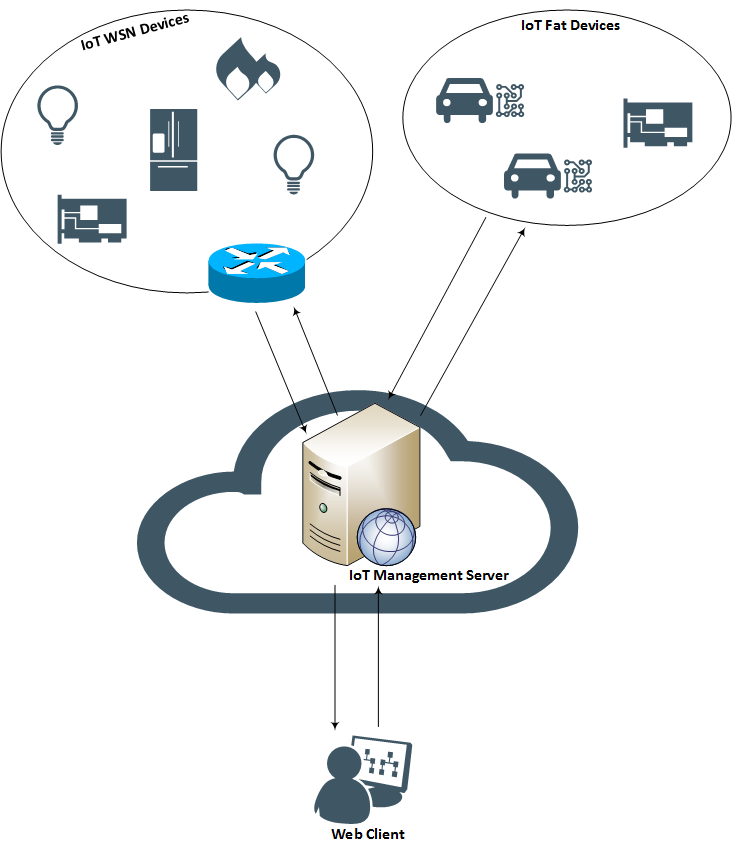
\includegraphics[scale=0.6]{../03_Design/images/systemuebersicht.png}\caption{Systemübersicht}
\end{figure}

\newpage


\begin{landscape}
\section{Klassenstruktur}
\subsection{Klassendiagramm}
\begin{figure}[H]
\centering
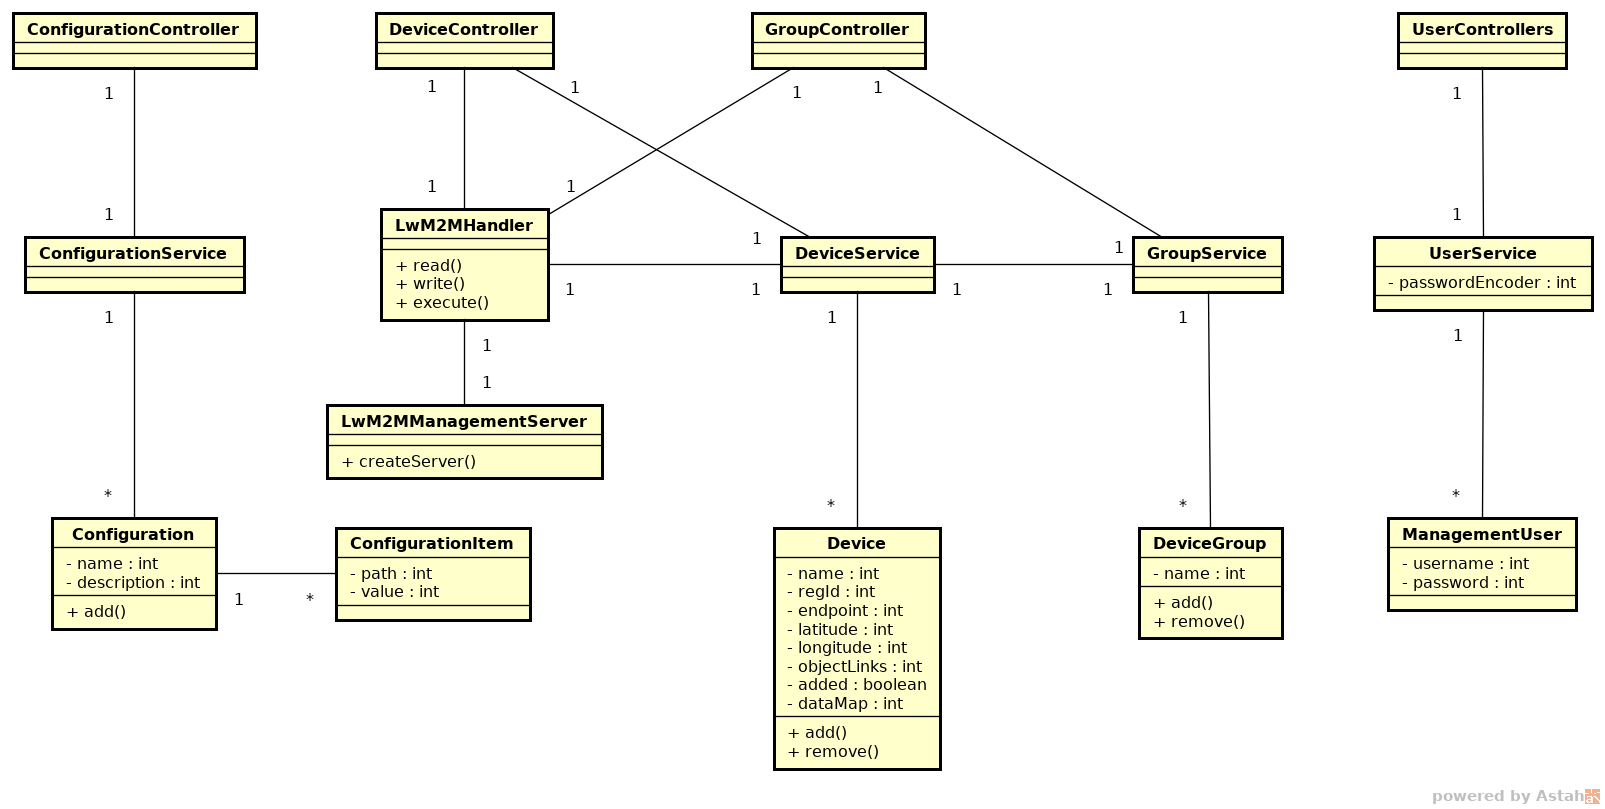
\includegraphics[width=1\textwidth]{../03_Design/images/domainmodel.png}
\caption{Klassendiagramm}
\end{figure}
\end{landscape}

\section{Logische Architektur}
\begin{figure} [H]
	\begin{center}
	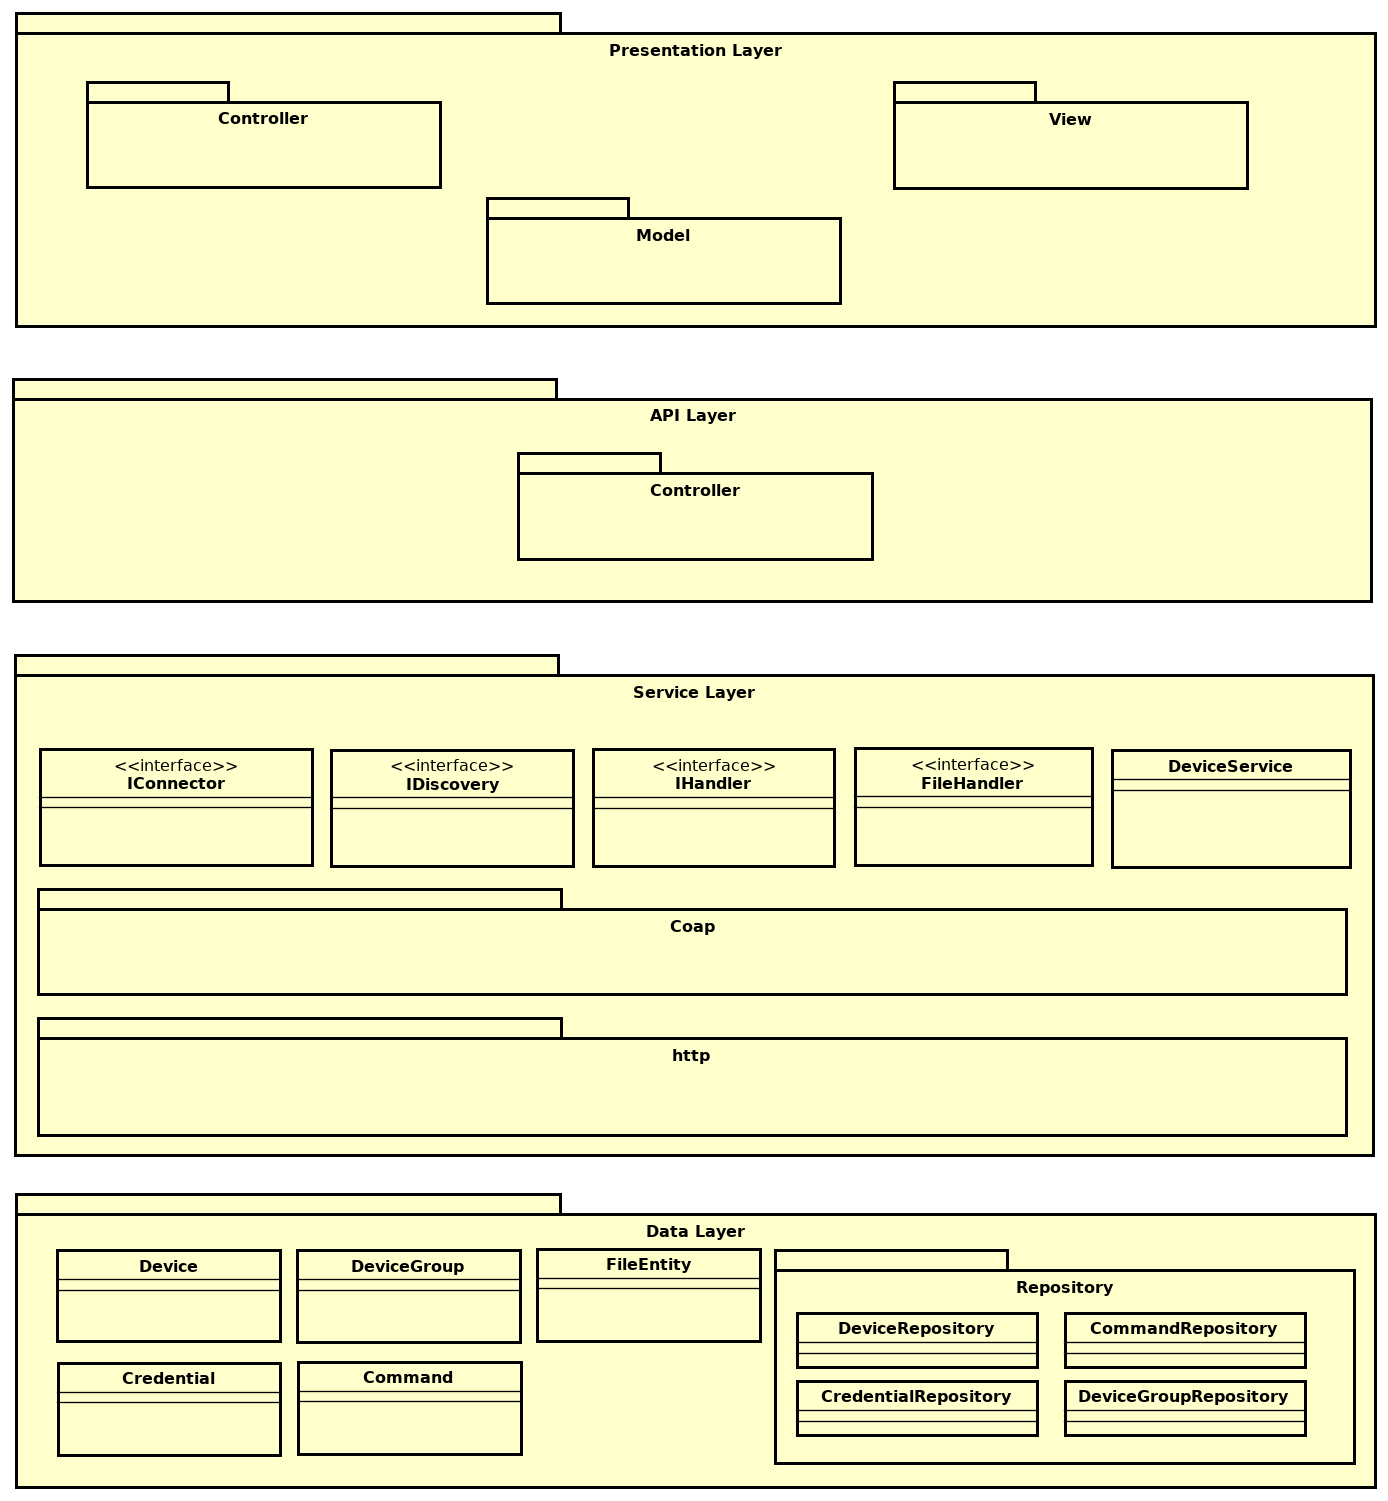
\includegraphics[width=0.90\textwidth]{../03_Design/images/architektur.png}
	\caption{Logische Architektur}
	\end{center}
\end{figure}

\newpage

\subsection{Presentation Layer}


Im Presentation-Layer gibt es Web-Controller und Rest-Controller. Die Web-Controller liefern die HTML-Inhalte aus. Die Rest-Contoller liefern Daten im JSON-Format oder es werden Methoden aus dem Service Layer gestartet, um die Daten zu verarbeiten.


\subsubsection{Packagestruktur}


\begin{table}[H]
\centering
    \begin{tabular}{@{}l p{11.9cm} @{}}\toprule    
    {Packagename} & {Beschreibung}\\ \midrule
    webcontrollers & Alle HTML-Inhalte werden durch die Web-Controller ausgeliefert. Dazu werden die Daten aus dem Service-Layer geholt.\\       
    restcontrollers & Die Rest-Controller führen Methoden auf dem Service-Layer aus und geben die Resultate als JSON zurück an den Client. \\
    \bottomrule
    \end{tabular}
\end{table}

\subsubsection{Klassenstruktur}

\begin{table}[H]
\centering
    \begin{tabular}{@{}l p{11.9cm} @{}}\toprule    
    {Klassenname} & {Beschreibung}\\ \midrule
     FrontWebController & Beinhaltet die Login, Logout und Home Routen.  \\       
     GroupWebController & Liefert alle für Groups relevanten HTML-Inhalte aus. \\       
     DeviceWebController & Liefert alle für Devices HTML-Inhalte aus.  \\       
     DiscoveryWebController & Beinhaltet die Discovery Routen.  \\       
     ConfigurationWebController & Beinhaltet die für die Configuration wichtigen Routen.  \\       
     UserWebController & Liefert die User HTML-Inhalte aus. \\       
     DeviceRestController & Führt Service-Layer Methoden aus und liefert JSON Daten.  \\       
     GroupRestController & Führt Service-Layer Methoden aus und liefert JSON Daten.  \\       
     ConfigurationRestController & Führt Service-Layer Methoden aus und liefert JSON Daten. \\       
     UserRestController & Führt Service-Layer Methoden aus und liefert JSON Daten.  \\         
    \bottomrule
    \end{tabular}
\end{table}

\subsubsection{Schnittstellen}
Der Presentation-Layer hat eine Schnittstelle zum Service-Layer. Alle Daten werden über den Service-Layer geholt und an den Service-Layer gegeben. So ist eine saubere Trennung zwischen Daten und Methoden sichergestellt. 

\newpage

\subsection{Service-Layer}
Der Service-Layer beinhaltet die Klassen, welche für die Verarbeitung der Daten zuständig ist. Hier werden alle Devices erfasst, verbunden und verwaltet. Dazu wird jedes gefundene Device auf der Datenbank hinterlegt. Bei einem Read, Write oder Execute wird das Device aus dem Data Layer geholt und mit den neuen Daten aktualisiert. Dabei wird hier zwischen Applikation-Services und LwM2M-Services unterschieden.

\subsubsection{Packagestruktur}

\begin{table}[H]
\centering
    \begin{tabular}{@{}l p{11.9cm} @{}}\toprule    
    {Packagename} & {Beschreibung}\\ \midrule
    applicationservice & Dieses Package beinhaltet die Klassen, welche die Devices oder Groups erstellen, anpassen usw. \\       
    lwm2mservices & Dieses Package beinhaltet alle Kommunikationsrelevanten Klassen, um mit den Devices Daten auszutauschen. \\
    \bottomrule
    \end{tabular}
\end{table}

\subsubsection{Klassenstruktur}
\begin{table}[H]
\centering
    \begin{tabular}{@{}l p{11.9cm} @{}}\toprule    
    {Klassenname} & {Beschreibung}\\ \midrule
     DeviceService & Holt und speichert die Devices von dem Data-Layer und verarbeitet die Änderungen  \\       
     GroupService & Zugriff auf den Data-Layer. Liest und schreibt alle Groups.  \\       
     ConfigurationService & Zugriff auf den Data-Layer. Liest und schreibt alle Configurationen.  \\  
     UserService & Checkt bei den Logins und verarbeitet die User Schreib- und Lesevorgänge.  \\            
     LocationService & Liest die Locations aus den Devices und gibt sie dem Controller weiter.  \\       
     InfrastructureService & Infrastruktur-Methoden, wie zum Beispiel Server-Uptime.  \\       
     LwM2MHandler & Beinhaltet alle Kommunikation zwischen Devices und dem Management Server.  \\       
     LwM2MManagementServer & Der Server, welche die Befehle aufs Netzwerk schickt und empfängt.  \\       
    \bottomrule
    \end{tabular}
\end{table}
\subsubsection{Schnittstellen}
Der Service-Layer hat eine Schnittstelle zum Data-Layer. Durch den Service-Layer werden die Datenobjekte erstellt, bearbeitet und ausgewertet. Der Presentation-Layer muss immer über den Service-Layer, um eine saubere Abtrennung der Schichten zu gewährleisten.

\newpage

\subsection{Data-Layer}
Der Data-Layer beinhaltet alle Datenobjekte, welche vom laufenden Programm benötigt werden. Diese werden von hier in die Datenbank geschrieben. Das Repository bietet die Datenbankmethoden an, um die Daten in die Datenbank zu speichern.

\subsubsection{Packagestruktur}
\begin{table}[H]
\centering
    \begin{tabular}{@{}l p{11.9cm} @{}}\toprule    
    {Packagename} & {Beschreibung}\\ \midrule
    repositories & Zugriffsmethoden auf die Datenbank. Eigene sowie durch die Library ausgelieferte Methoden. \\       
    \bottomrule
    \end{tabular}
\end{table}

\subsubsection{Klassenstruktur}
\begin{table}[H]
\centering
    \begin{tabular}{@{}l p{11.9cm} @{}}\toprule    
    {Klassenname} & {Beschreibung}\\ \midrule
    Device & Device ist eine Datenklasse, welche alle Daten von einem Device beinhaltet.\\
    DeviceGroup & In der Datenklasse DeviceGroup, werden alle Gruppen verwaltet, damit das Composite-Pattern umgesetzt werden kann.\\
    ManagementUser & Datenklasse für die Loginbenutzer.\\
    Configuration & Configuration Datenklasse, welche eine List von ConfigurationItems beinhaltet. \\
    ConfigurationItem & Datenklasse für die einzelnen ConfigurationItems.\\
    \bottomrule
    \end{tabular}
\end{table}
\subsubsection{Schnittstellen}
Da der Data-Layer die unterste Schicht ist, gibt es nur eine Verbindung zur Datenbank.

\newpage

\section{Deployment}
Die Applikation hat eine typische 3-Tier Architektur. Es wird ein Serverseitiges Templating verwendet. Alle Daten werden daher auf dem Server verarbeitet und als HTML an den Client gesendet. Die Daten werden in einer Datenbank persistiert.
\begin{figure}[H]
\center
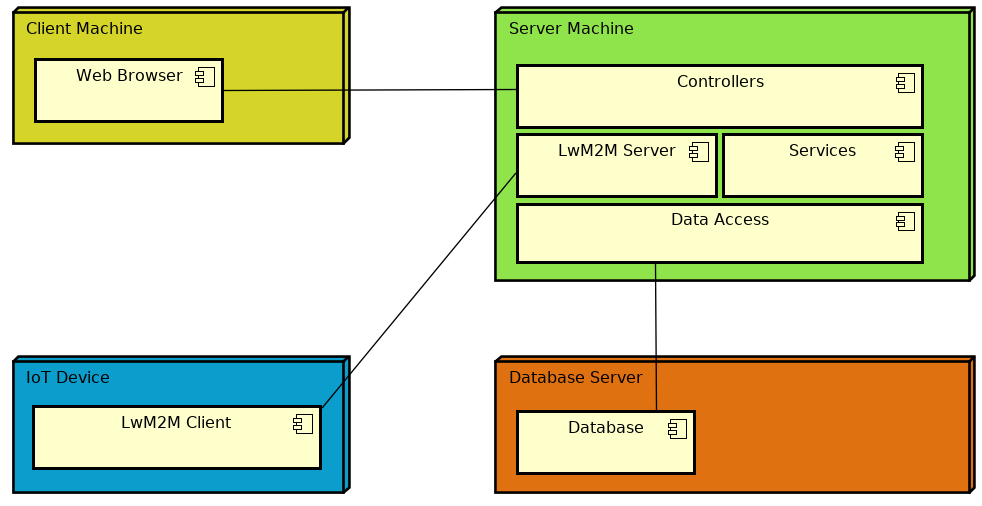
\includegraphics[scale=0.6]{../03_Design/images/architekturuebersicht}\caption{Deployment}
\end{figure}

\section{User Interface Entwurf}
\label{sec:mockups}
\subsection{Design}
Das Projekt erhält eine möglichst einfach gehaltene Benutzeroberfläche. Durch die farbliche Trennung von Funktionen und fixen Bereichen für die Daten, soll die Oberfläche einfach und intuitiv gestaltet werden. Zusätzlich wird die Oberfläche responsiv aufgebaut, damit sie an unterschiedlichen Bildschirmgrössen verwendbar wird.

Es wurden Mock-ups anhand von einfachen Handskizzen erstellt, um das aussehen und die Funktionen der Benutzeroberfläche zu planen.

\subsection{Ansichten}
\subsubsection{Startseite}
\begin{figure} [H]
	\begin{center}
	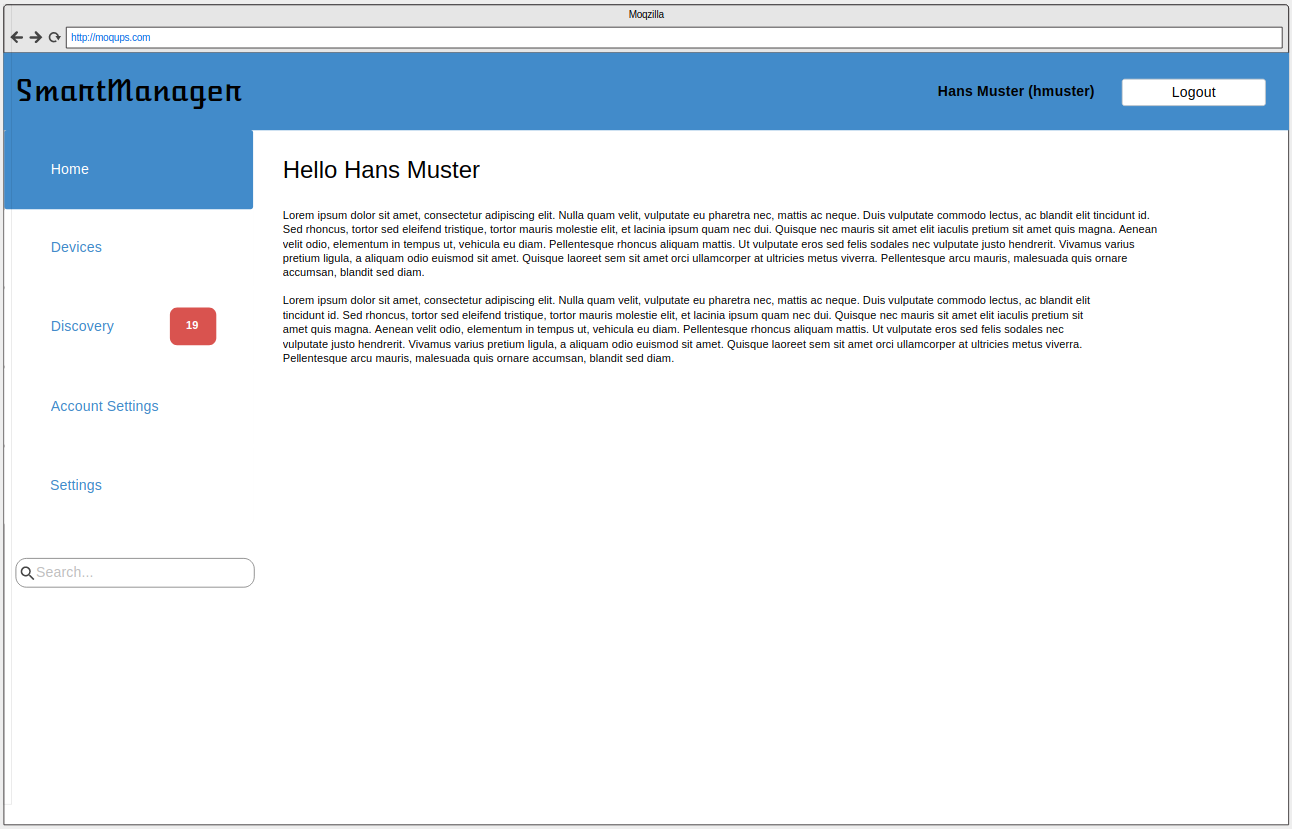
\includegraphics[width=0.80\textwidth]{../03_Design/images/home.png}
	\caption{Startseite}
	\end{center}
\end{figure}
Die Startseite zeigt dem Benutzer Hilfestellungen an und führt den Benutzer durch die ersten Schritte. Auf der Linken Seite befindet sich das Menu und eine Suche. Oben Rechts findet der Benutzer den Loginbereich und die Benutzerangaben.

Beim Menu gibt es statische, sowie dynamische Einträge. Der Discoveryeintrag ist ein dynamischer Eintrag und zeigt die Anzahl gefundenen Geräte an.

\subsubsection{Device List}
\begin{figure} [H]
	\begin{center}
	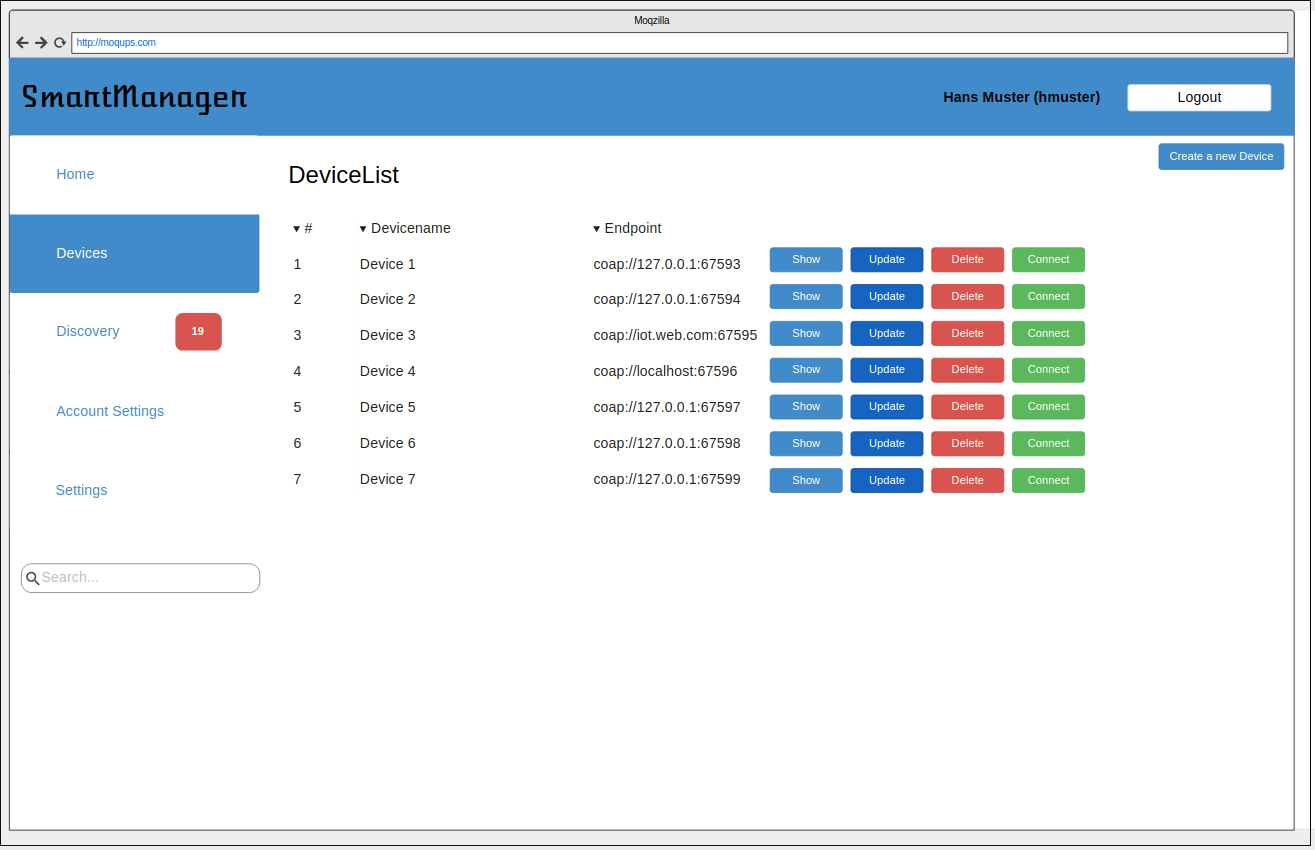
\includegraphics[width=0.80\textwidth]{../03_Design/images/devicelist.png}
	\caption{Device List}
	\end{center}
\end{figure}
In der Device Liste werden alle Devices angezeigt. Dazu wird zu jedem Device die jeweiligen Möglichkeiten als Button eingeblendet. So kann man ein Device betrachten, Anpassen, Löschen und sich mit dem Gerät verbinden. Zusätzlich werden die Daten, wie zum Beispiel Endpoint angezeigt.

Oben rechts befindet sich der Button, um weitere Devices zu erstellen.
\begin{description}
\item [Show] Zeigt die Details zu einem Device an
\item [Update] Führt zum Device Update Formular, damit das Device angepasst werden kann.
\item [Delete] Button, der das Device aus der Applikation löscht
\item [Connect] Button, um sich mit dem Gerät zu verbinden.
\item [Create a new Device] Führt zur Create Device Ansicht.
\end{description}


\subsubsection{Create Device}
\begin{figure} [H]
	\begin{center}
	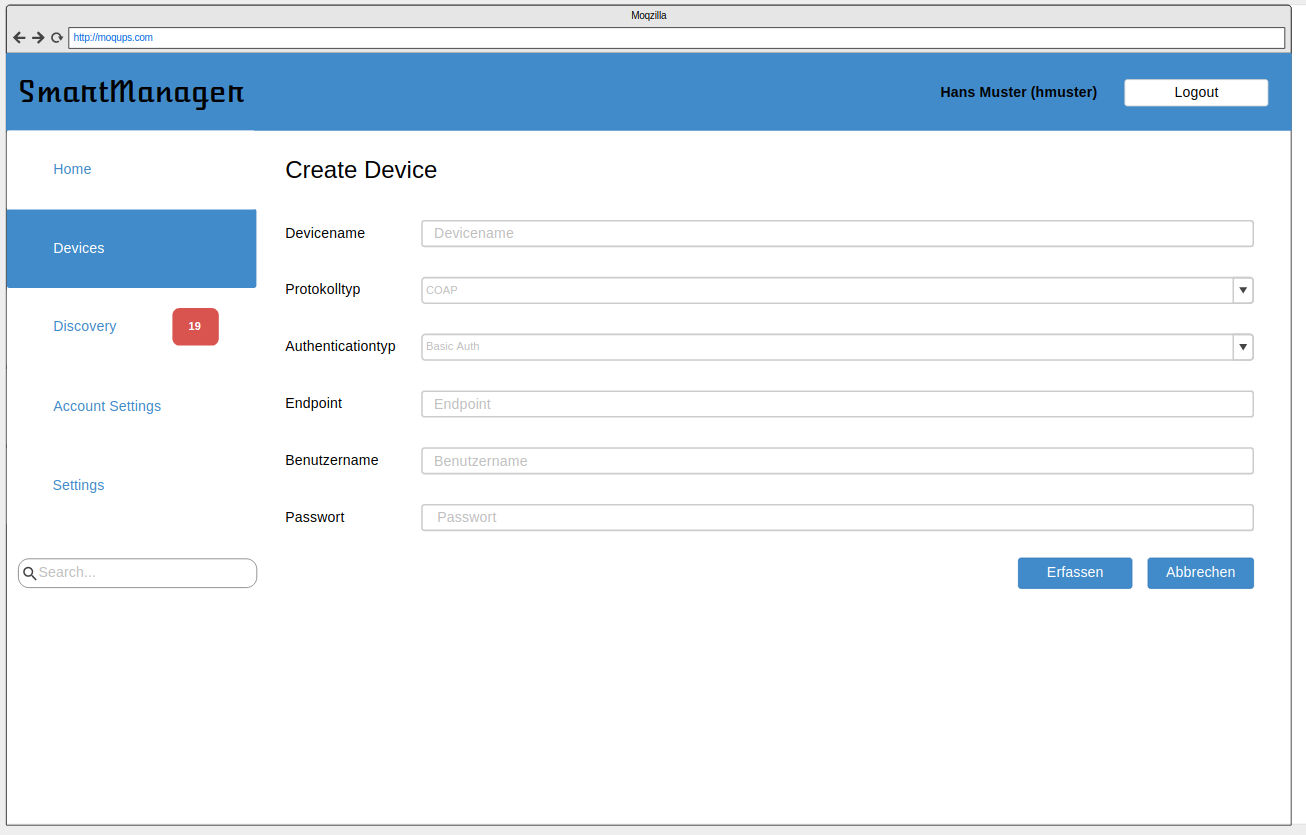
\includegraphics[width=0.80\textwidth]{../03_Design/images/createdevice.png}
	\caption{Create Device}
	\end{center}
\end{figure}
Bei der Create Device Ansicht kann ein neues Device erstellt werden. Dadurch wird das Device manuell erfasst und in der Datenbank abgelegt. Dies kann gemacht werden, wenn das Device nicht via Discovery gefunden worden ist.

Je nach Combobox Auswahl passt sich das Formular an, um zum Beispiel auch Zertifikate hinterlegen zu können.

\begin{description}
\item [Erfassen / Update] Erstellt oder passt ein Device an
\item [Abbrechen] Bricht den Device Create ab und führt zur Device List Ansicht
\end{description}

\subsubsection{Device Details}
\begin{figure} [H]
	\begin{center}
	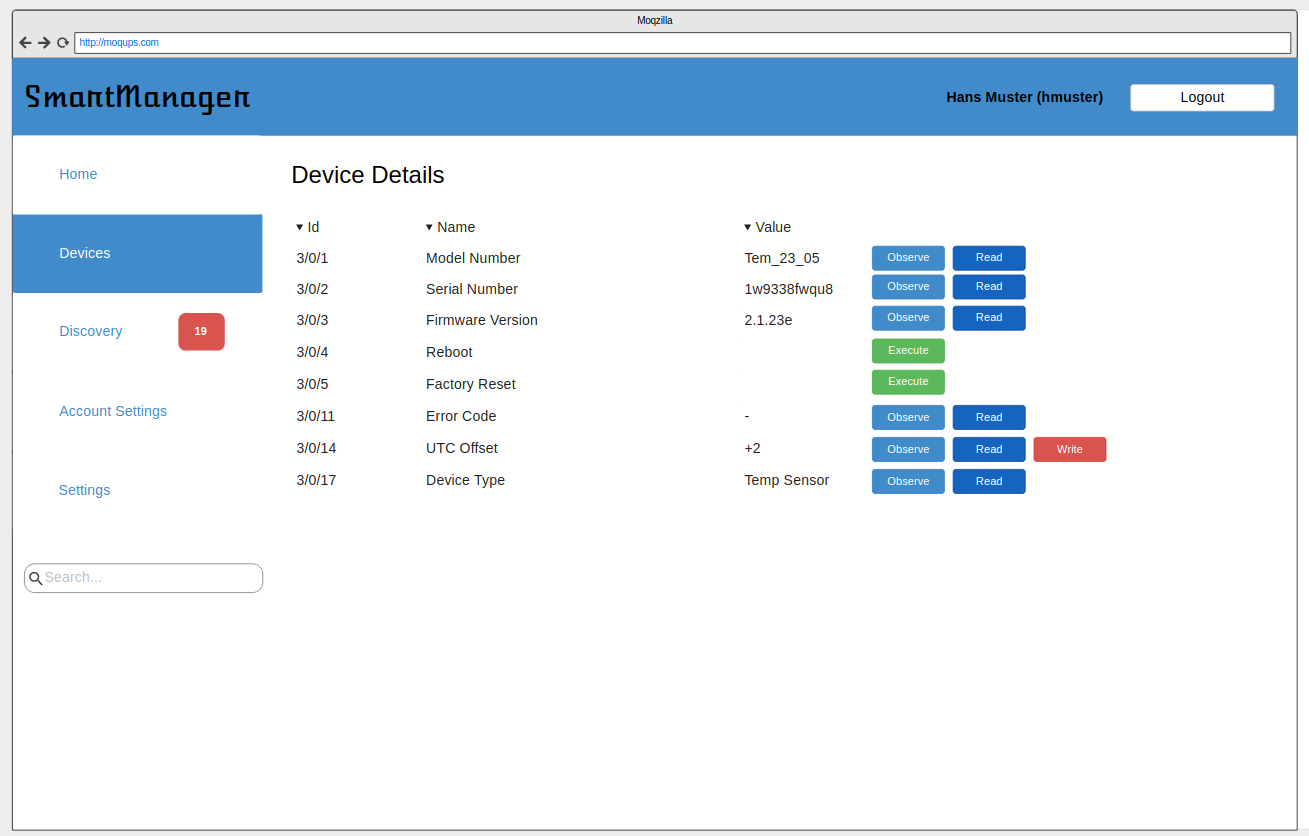
\includegraphics[width=0.80\textwidth]{../03_Design/images/devicedetails.png}
	\caption{Device Details}
	\end{center}
\end{figure}
Alle wichtige Informationen eines Devices werden in dieser Übersicht angezeigt. Zu Jeder Ressource wird die Id, der Name und den aktuellen Wert angezeigt. Je nach Ressource passen sich die Möglichen Aktionen an. Dabei gibt es Observe, Read, Write und Execute. Bei Write wird ein zusätzliches Eingabefeld eingeblendet, um den gewünschten Wert eintragen zu können.

\begin{description}
\item [Observe] Startet ein Observer für die gewünschte Ressource.
\item [Read] Liest die Ressource vom Device
\item [Write] Schreibt den Wert in die Ressource und aktualisiert den Eintrag in der Datenbank
\item [Execute] Führt einen Befehl auf dem Device aus
\end{description}

\subsubsection{Discover Device}
\begin{figure} [H]
	\begin{center}
	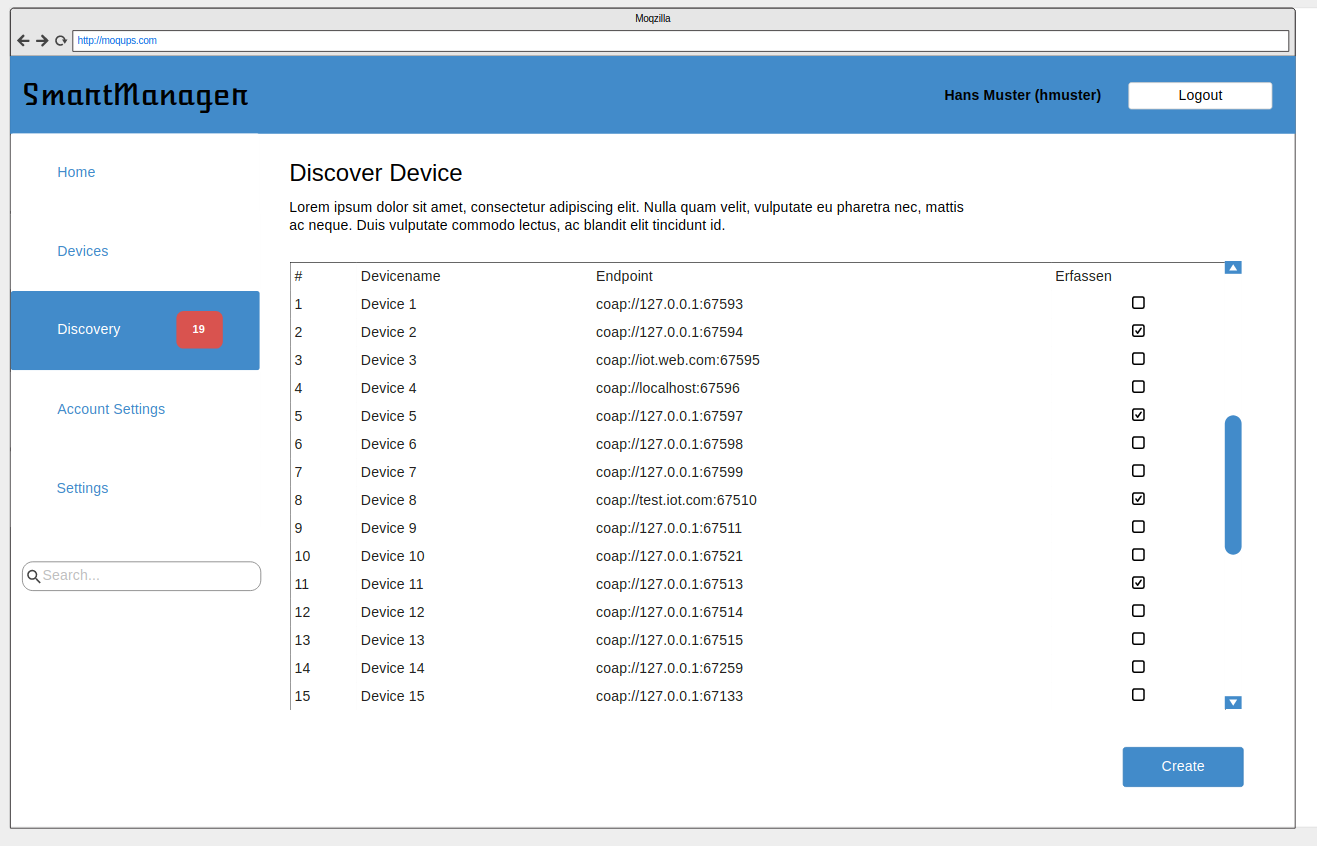
\includegraphics[width=0.80\textwidth]{../03_Design/images/devicediscover.png}
	\caption{Device Details}
	\end{center}
\end{figure}
Alle durch das Discovery gefundenen Devices werden in dieser Übersicht aufgelistet. Dazu werden direkt die wichtigen Daten angezeigt und man hat die Möglichkeit das gewünschte Device zur Applikation hinzuzufügen. Die Anzahl gefundenen Devices werden auf der Linken Seite im Menu angezeigt und passt sich dynamisch an.

\begin{description}
\item [Create] Erstellt für die ausgewählten Devices ein Deviceobjektauf der Datenbank
\end{description}